\documentclass{article}

\usepackage[left=2cm,right=2cm,top=2cm,bottom=2cm]{geometry} 

\usepackage[utf8]{inputenc}   % otra alternativa para los caracteres acentuados y la "ñ"
\usepackage[           spanish % para poder usar el español
                      ,es-tabla % para los captions de las tablas
                       ]{babel}   
\decimalpoint %para usar el punto decimal en vez de coma para los números con decimales

%\usepackage{beton}
%\usepackage[T1]{fontenc}

\usepackage{parskip}
\usepackage{xcolor}

\usepackage{caption}

\usepackage{fancyvrb}

\usepackage{enumerate} % paquete para poder personalizar fácilmente la apariencia de las listas enumerativas

\usepackage{graphicx} % figuras
\usepackage{subfigure} % subfiguras

\usepackage{amsfonts}
\usepackage{amsmath}

\usepackage[formats]{listings}
\lstdefineformat{R}{~=\( \sim \)}
\lstset{basicstyle=\ttfamily,format=R}

\definecolor{gris}{RGB}{220,220,220}
	
\usepackage{float} % para controlar la situación de los entornos flotantes

\restylefloat{figure}
\restylefloat{table} 
\setlength{\parindent}{0mm}


\usepackage[bookmarks=true,
            bookmarksnumbered=false, % true means bookmarks in 
                                     % left window are numbered
            bookmarksopen=false,     % true means only level 1
                                     % are displayed.
            colorlinks=true,
            allcolors=blue,
            urlcolor=blue]{hyperref}
\definecolor{webblue}{rgb}{0, 0, 0.5}  % less intense blue


\title{\Huge SWAP: Replicación de bases de datos MySQL\vspace{10mm}}

\author{\huge David Cabezas Berrido \vspace{10mm} \\ 
  \huge dxabezas@correo.ugr.es \vspace{10mm}}

\begin{document}
\maketitle
\tableofcontents
\newpage

\section{Preparativos}

Es importante desactivar el cortafuegos antes de hacer la configuración de maestro-esclavo. Como medida preventiva, desactivamos el 
cortafuegos en
todas las máquinas ejecutando el script \texttt{off.sh} de la práctica anterior (para \emph{iptables}) y también \verb|sudo ufw disable| (para UFW).

\section{Base de datos MySQL}

Creamos la base de datos, la tabla e insertamos una tupla tal y como se describe en el guión.

Como opción avanzada, podemos exigir que algún campo no pueda ser nulo, por ejemplo el campo usuario. Esto se consigue
añadiendo \texttt{NOT NULL} detás del tipo del campo. Además, a la hora de insertar una tupla podemos omitir el nombre de los atributos si
 ponemos los valores en el mismo orden que aparecen en la descripción (el orden que usamos cuando creamos la tabla), aunque esto
 no es muy recomendable (si se modificase la tabla, habría que cambiar los scripts de inserción en caso de tenerlos).
 
\begin{figure}[H]
	\centering
	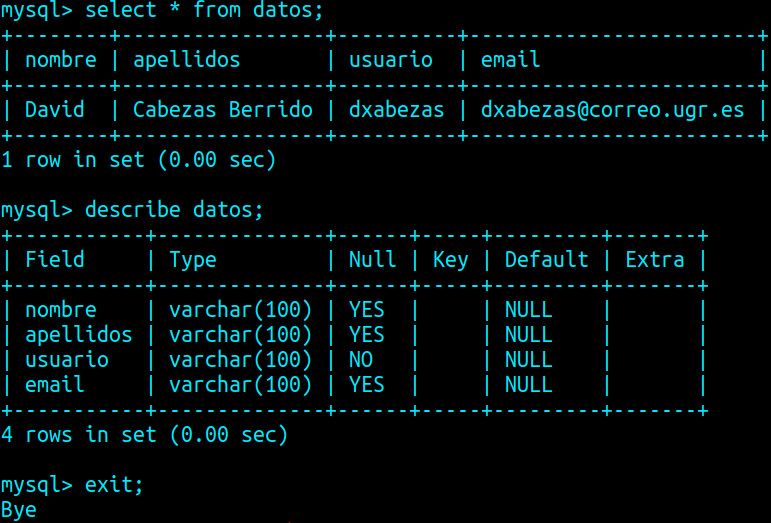
\includegraphics[width=120mm]{imgs/mydb}
	\caption{Tenemos una tupla en la tabla que hemos creado. En la descripción de la tabla podemos ver los distintos
	campos y el tipo de cada uno. Nos fijamos que el campo usuario no puede ser nulo.}
	\label{fig:mydb}
\end{figure}

\subsection{Replicar la BD con mysqldump}

Antes de realizar la copia, debemos bloquear las tablas.

\begin{figure}[H]
	\centering
	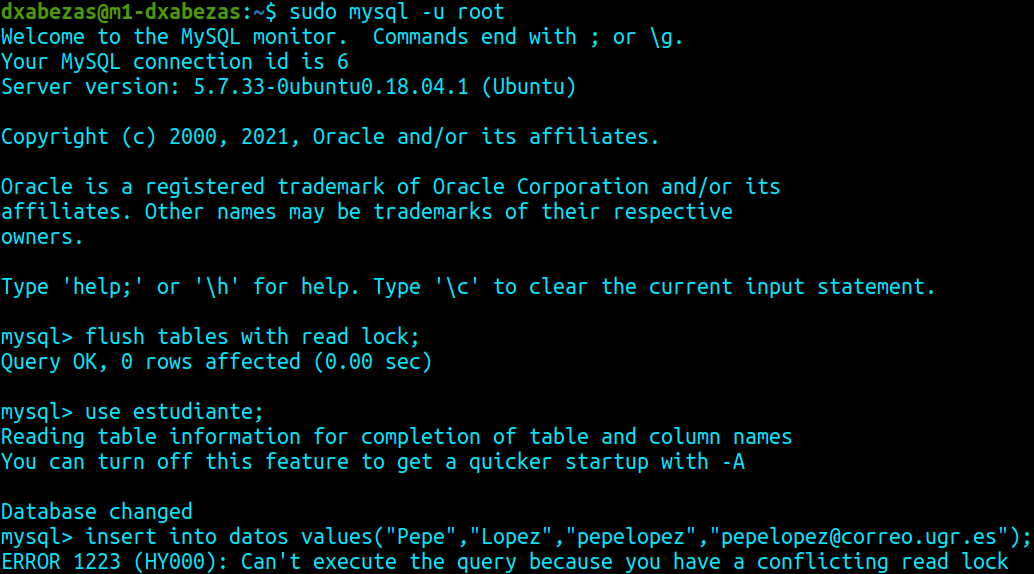
\includegraphics[width=150mm]{imgs/lock}
	\caption{Bloqueamos las tablas y comprobamos que no se puede modificar la base de datos.}
	\label{fig:lock}
\end{figure}

Ahora desde bash copiamos la base de datos a un archivo con
\begin{Verbatim}
sudo mysqldump estudiante -u root > /tmp/estudiante.sql
\end{Verbatim}
Después volvemos a entrar a MySQL y desbloqueamos las tablas con \verb|unlock tables;|.

\end{document}
